\documentclass{article}
\usepackage{amsmath}
\usepackage{amssymb}
\usepackage{indentfirst}
\usepackage{graphicx}
\usepackage{color}
\usepackage{fancyhdr}
\usepackage{epstopdf}
\usepackage{indentfirst}
\usepackage{geometry}
\geometry{left=2.5cm,right=2.5cm,top=2.5cm,bottom=2.5cm}

\title{14.03 Problem Set 3}
\author{Yijun Jiang}
%\email{yjjiang@mit.edu}
\date{\today}

\pagestyle{fancy}
\lhead{Yijun Jiang}
\rhead{14.03 Problem Set 3}

\begin{document}
\maketitle

\section{Tariffs and Quotas}
\subsection{Part 1}
If US does not trade with the rest of world, domestic demand should balance domestic supply.
\begin{align*}
	&P=2+Q\\
	&Q=-\frac{1}{3}P+6
\end{align*}
whose solution is $P^*=6$ and $Q^*=4$. This is the equilibrium price and quantity in autarky.

\subsection{Part 2}
The new supply curve first goes as $P=2+Q$ and then becomes perfectly elastic at $P=3$. Once $Q$ is large enough to make $P=3$, Chinese suppliers enter the market and fixes market price at $P=3$. For US suppliers, only those who are willing to supply at $P\leqslant3$ can survive in this market. In the previous part we find that $P=6>3$. Therefore, we know that Chinese suppliers do enter the market. The new equilibrium price is then $P^*=3$, both for US and Chinese suppliers. The equilibrium quantity is given by the domestic demand function, $Q^*=-\frac{1}{3}P+6=5$.

At the turning point where Chinese suppliers enter the market, $Q^*_{US}=P^*-2=1$. This is the quantity produced by US suppliers. The rest of the demand, $Q^*_{CHN}=Q^*-Q^*_{US}=4$, is imported from Chinese suppliers.

\subsection{Part 3}
This tariff effectively sets the Chinese supply curve to $P=3+t=4.5$, which is still lower than $P=6$ found in part 1. So Chinese suppliers still enter the market and market price will be fixed at $P^*=4.5$, but more US suppliers can sell their T-shirts at this higher price. Numerically, $Q^*_{US}=P^*-2=2.5$.

In conclusion, the equilibrium price and quantity sold by US manufacturers are now $P^*=4.5$ and $Q^*_{US}=2.5$. So $\Delta P^*=1.5$ and $\Delta Q^*_{US}=1.5$.

\subsection{Part 4}
The US manufacturers who can supply below $P=3$ (low-cost US suppliers) enter the market first, then Chinese suppliers, and finally, when the import quota is used up but consumers still demand more T-shirts, the price is raised above $P=3$ and the rest US suppliers (high-cost US suppliers) enter the market.

In order to maintain the domestic production level, the equilibrium price must be $P^*=2+Q^*_{US}=4.5$. At this price, domestic demand is $Q^*=-\frac{1}{3}P+6=4.5$. So the quota must be set as $Q^*_{CHN}=Q^*-Q^*_{US}=2$.

\subsection{Part 5}
See Fig.\ref{DandS} for the graph.
\begin{figure}[!htbp]
	\centering
	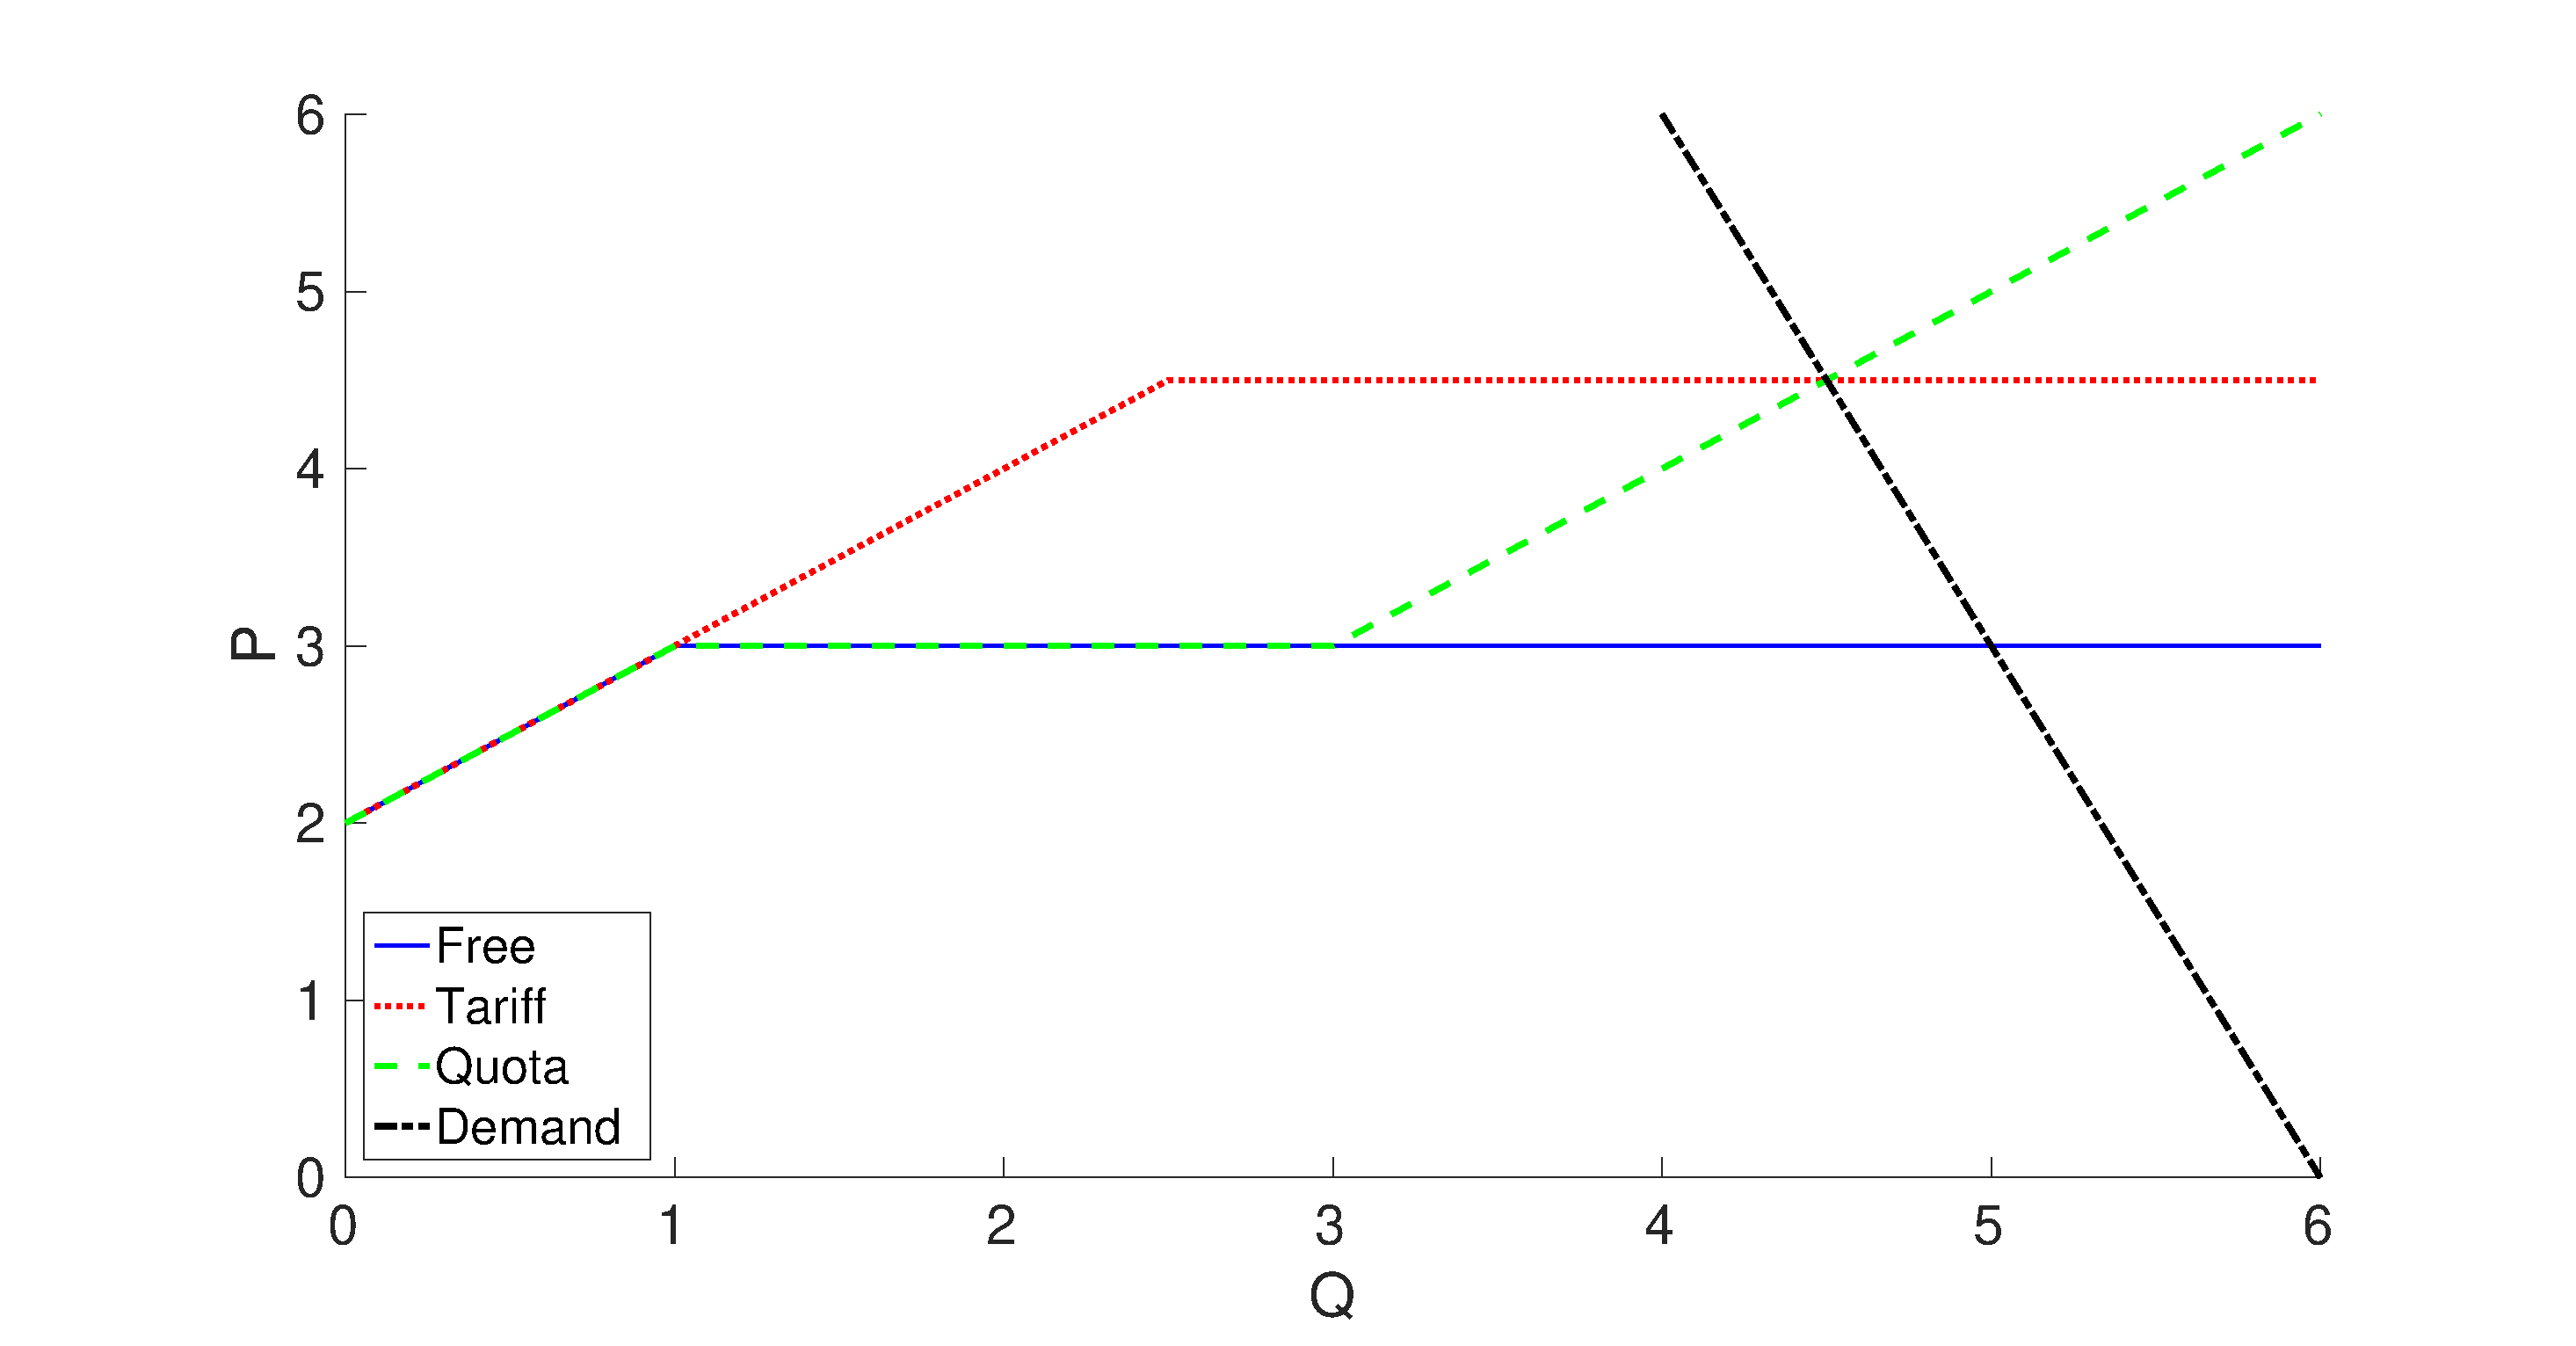
\includegraphics[width=12cm]{figure1.eps}\\
	\caption{Demand and supply curves of free trade and trade with tariff or quota}
	\label{DandS}
\end{figure}

\subsection{Part 6}
See Fig.\ref{surplus} for a graphical illustration.
\begin{figure}[!htbp]
	\centering
	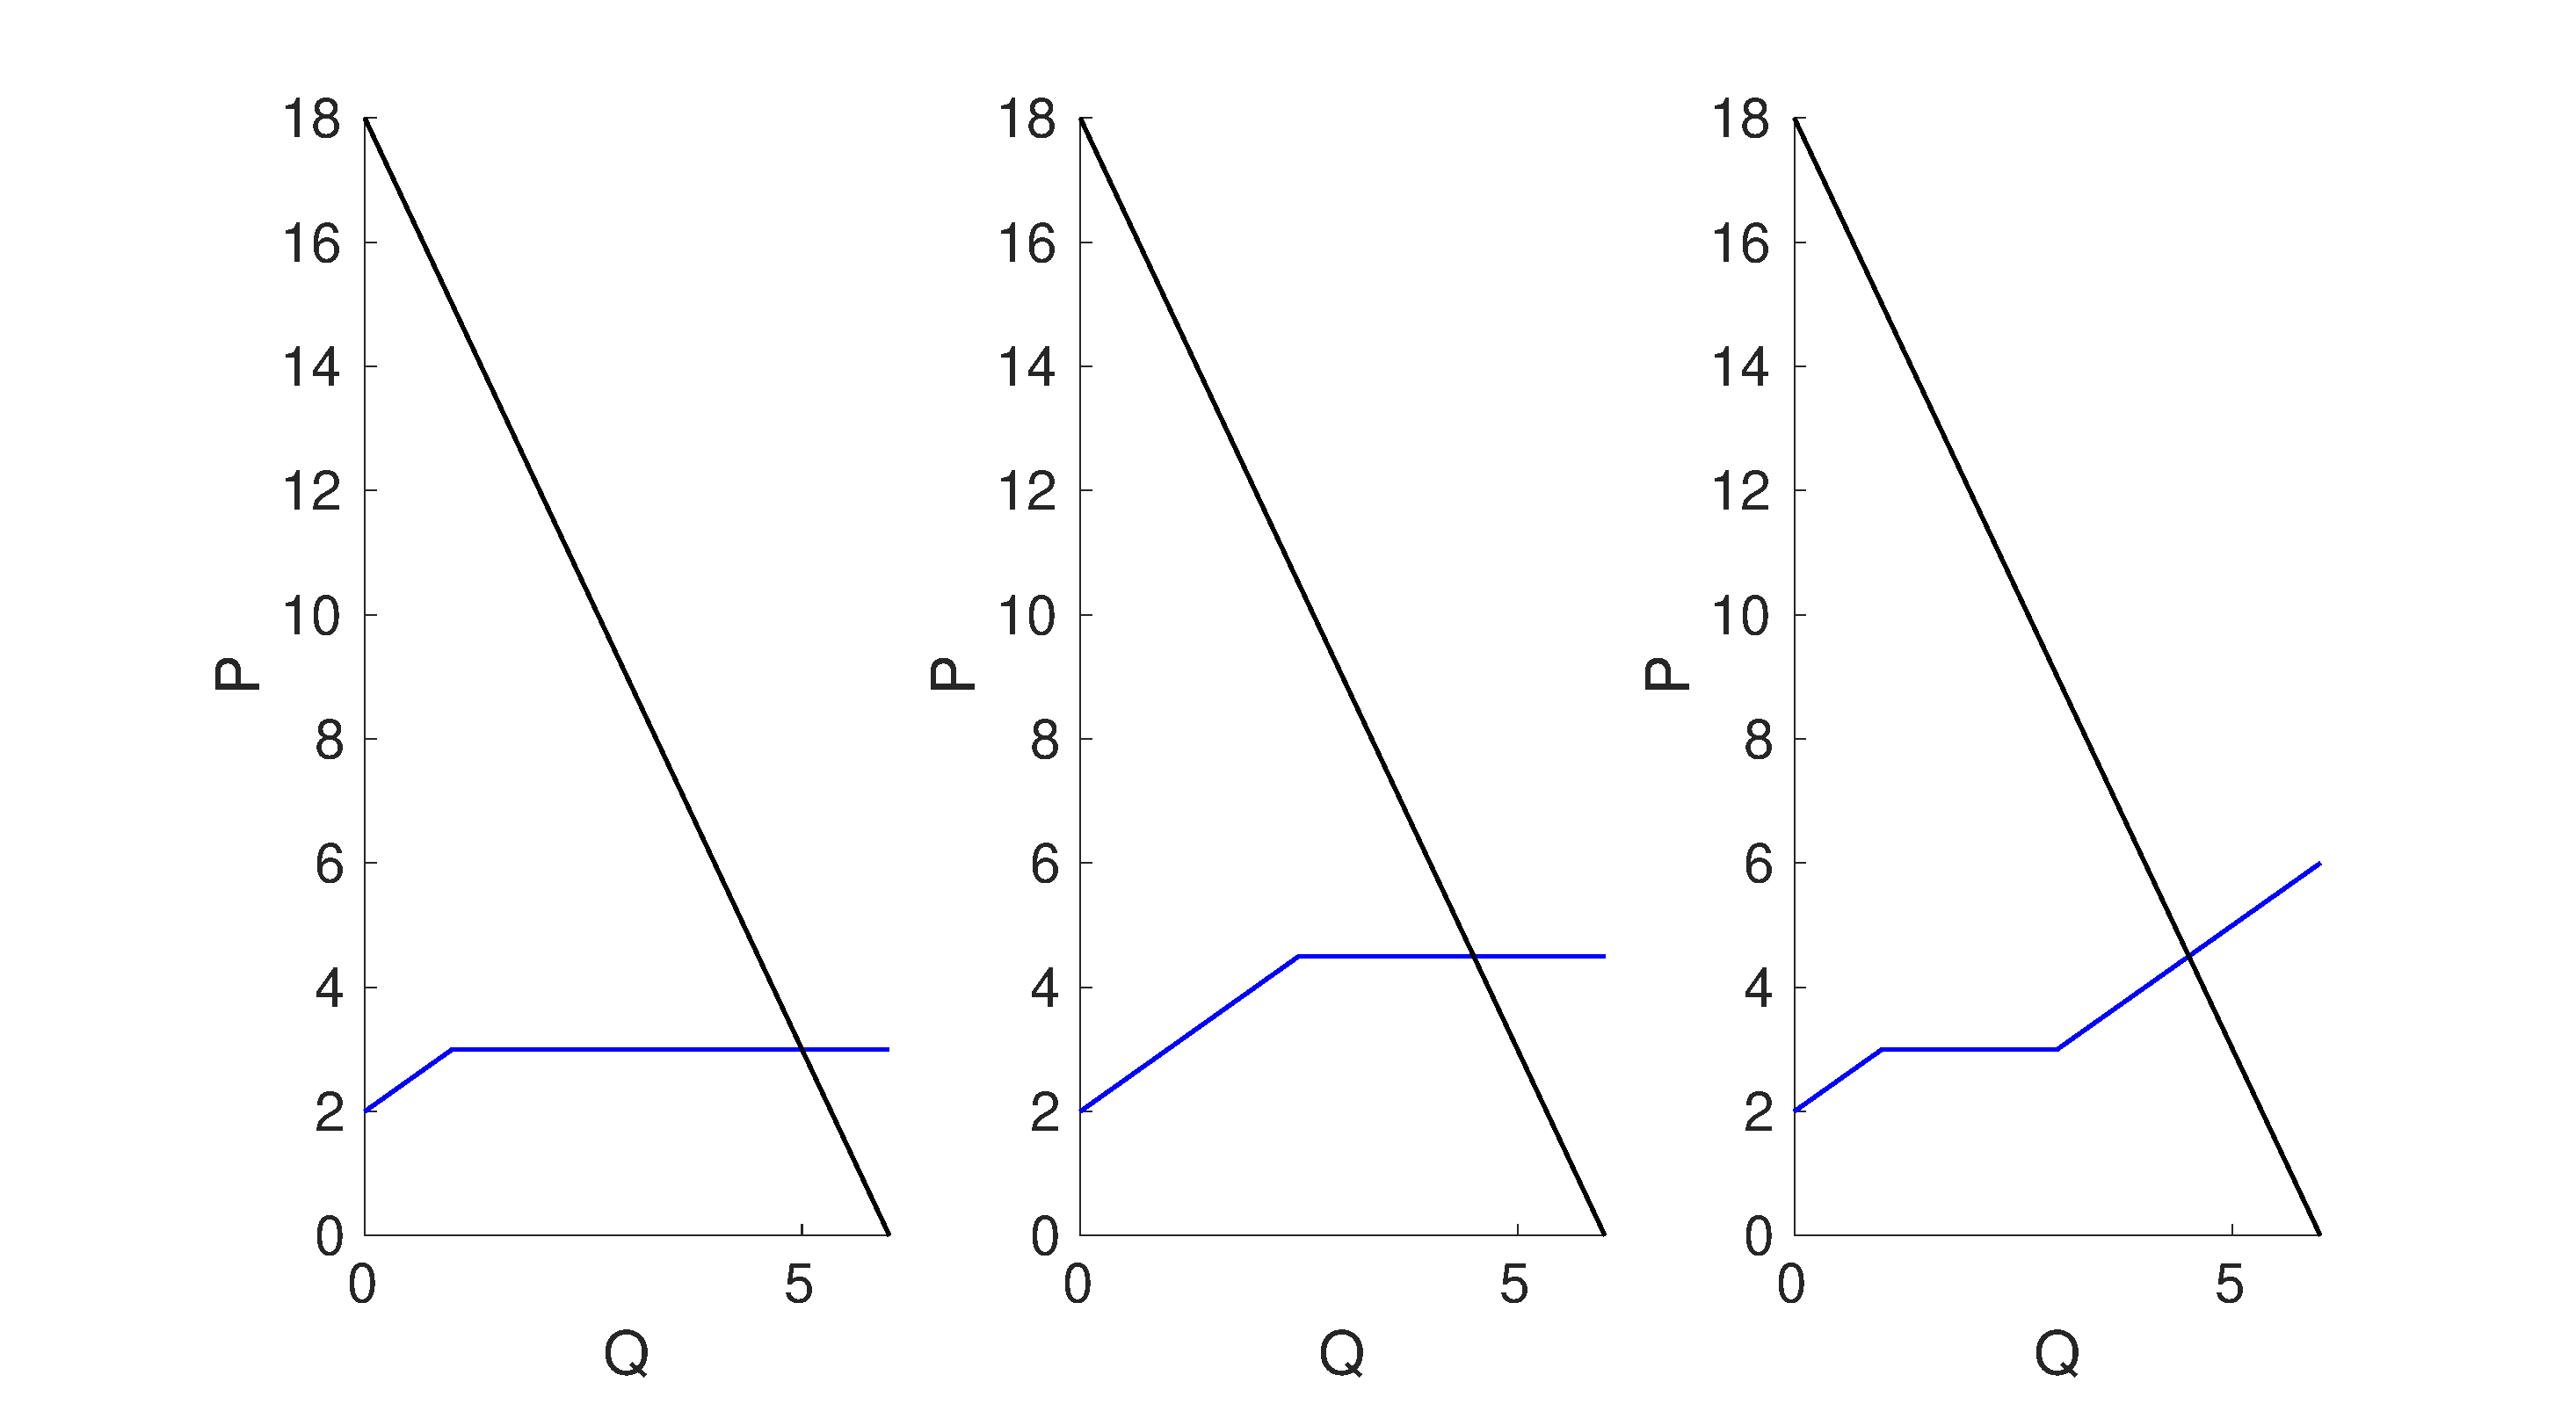
\includegraphics[width=12cm]{figure2.eps}\\
	\caption{Consumer and producer surplus of (left) free trade, (middle) trade with tariff, and (right) trade with quota}
	\label{surplus}
\end{figure}

In the free trade regime, consumer surplus is the area of the large triangle. US producer surplus is the area of the small triangle, while Chinese suppliers do not have any producer surplus. US government does not have any revenue.
\begin{align*}
	&CS_{free}=5\times(18-3)/2=37.5\\
	&PS_{US,free}=1\times(3-2)/2=0.5\\
	&PS_{CHN,free}=0\\
	&GR_{free}=0
\end{align*}

In the tariff regime, consumer surplus is the area of the large triangle. US producer surplus is the area of the small triangle, while Chinese suppliers do not have any producer surplus. US government revenue is the area of the rectangle.
\begin{align*}
	&CS_{tariff}=4.5\times(18-4.5)/2=30.375\\
	&PS_{US,tariff}=2.5\times(4.5-2)/2=3.125\\
	&PS_{CHN,tariff}=0\\
	&GR_{tariff}=(4.5-2.5)*(4.5-3)=3
\end{align*}


In the quota regime, consumer surplus is the area of the large triangle. US producer surplus has two parts on the graph: one for low-cost suppliers and the other for high-cost suppliers. Chinese producer surplus is the area of the rectangle. US government does not have any revenue.
\begin{align*}
	&CS_{quota}=4.5\times(18-4.5)/2=30.375\\
	&PS_{US,quota}=1\times((4.5-2)+(4.5-3))/2+(4.5-3)\times(4.5-3)/2=3.125\\
	&PS_{CHN,quota}=(3-1)\times(4.5-3)=3\\
	&GR_{quota}=0
\end{align*}

US consumers get the largest surplus in the free trade, so they prefer no import constraints. US producers regard both tariff and quota as better than free trade, and they are indifferent between tariff and quota policy, as long as the two policies give them the same market share. Chinese producers will prefer quota to tariff, for they get some producer surplus in the quota regime, which in the tariff regime turns into US government revenue.

\section{Deadweight Loss of Taxation}
\subsection{Part 1}
The utility maximization problem is
\begin{align*}
	&u^*=\max_{x,y}\{u(x,y)=x^{2/3}y^{1/3}\}\\
	&\textup{s.t. }xP_x+yP_y=I
\end{align*}

The Lagrangian is $L(x,y,\lambda)=x^{2/3}y^{1/3}+\lambda(I-xP_x-yP_y)$. Setting partial derivatives to zero,
\begin{align*}
	&\frac{2}{3}\left(\frac{x}{y}\right)^{-1/3}=\lambda P_x\\
	&\frac{1}{3}\left(\frac{x}{y}\right)^{2/3}=\lambda P_y\\
	&xP_x+yP_y=I
\end{align*}
whose solution is
\begin{align*}
	x&=\frac{2I}{3P_x}\\
	y&=\frac{I}{3P_y}\\
	\lambda&=\frac{1}{3}\left(\frac{1}{4}P_x^2P_y\right)^{-1/3}
\end{align*}

This gives the uncompensated demands,
\begin{align*}
	d_x(P_x,P_y,I)&=\frac{2I}{3P_x}\\
	d_y(P_x,P_y,I)&=\frac{I}{3P_y}
\end{align*}
as well as the indirect utility function,
\begin{equation*}
	V(P_x,P_y,I)=u(d_x,d_y)=\frac{2^{2/3}}{3}P_x^{-2/3}P_y^{-1/3}I
\end{equation*}

\subsection{Part 2}
Since utility remains the same, we have
\begin{equation*}
	V(P_x,P_y,I)=V(P_x(1+t),P_y,I+\delta I)
\end{equation*}

In other words,
\begin{align*}
	\frac{2^{2/3}}{3}P_x^{-2/3}P_y^{-1/3}I&=\frac{2^{2/3}}{3}(P_x(1+t))^{-2/3}P_y^{-1/3}(I+\delta I)\\
	\delta I&=\left((1+t)^{2/3}-1\right)I
\end{align*}

\subsection{Part 3}
\begin{align*}
	TR&=tP_x\cdot d_x(P_x(1+t),P_y,I+\delta I)\\
	&=tP_x\frac{2(I+\delta I)}{3P_x(1+t)}\\
	&=\frac{2I}{3}\frac{t}{(1+t)^{1/3}}
\end{align*}

\subsection{Part 4}
\begin{align*}
	DWL&=\delta I-TR\\
	&=\left((1+t)^{2/3}-1\right)I-\frac{2I}{3}\frac{t}{(1+t)^{1/3}}\\
	&=\frac{(1+t/3)-(1+t)^{1/3}}{(1+t)^{1/3}}I\\
	&=\frac{t^2/9-5t^3/81+O(t^4)}{(1+t)^{1/3}}I
\end{align*}

This deadweight loss is zero when $(1+t/3)=(1+t)^{1/3}$, which happens if and only if $t=0$. This is the trivial solution where no taxation exists. Nonzero tax always leads to a positive deadweight loss, for $(1+t/3)>(1+t)^{1/3}$ always holds when $t>0$. In other words, the government needs to rebate more than its tax revenue in order to make consumers equally satisfied as before.

\subsection{Part 5}
The diagram is shown in Fig.\ref{blank}, in which we can see that the cost of the new bundle at the original prices is higher than the original bundle. This intuitively makes sense because according to the dual problem, the original bundle minimizes the expenditure on this indifference curve. This statement is always true as long as $t>0$, so there is always some positive deadweight loss.
\begin{figure}[!htbp]
	\centering
	
\includegraphics[width=12cm]{blank.png}\\
	\caption{Graphical illustration of taxation and rebate}
	\label{blank}
\end{figure}

\section{General Equilibrium in a Pure Exchange Economy}
\subsection{Part 1}
The Edgeworth box is shown in Fig.\ref{Edgeworth}. Feasible allocations are all the points in the rectangular region $0\leqslant x\leqslant8$, $0\leqslant y\leqslant8$. If $x$ and $y$ must take integer values due to indivisibility of the goods, then feasible allocations are all the integer-coordinated grid points in this rectangle. The initial allocation is marked as a circle.
\begin{figure}[!htbp]
	\centering
	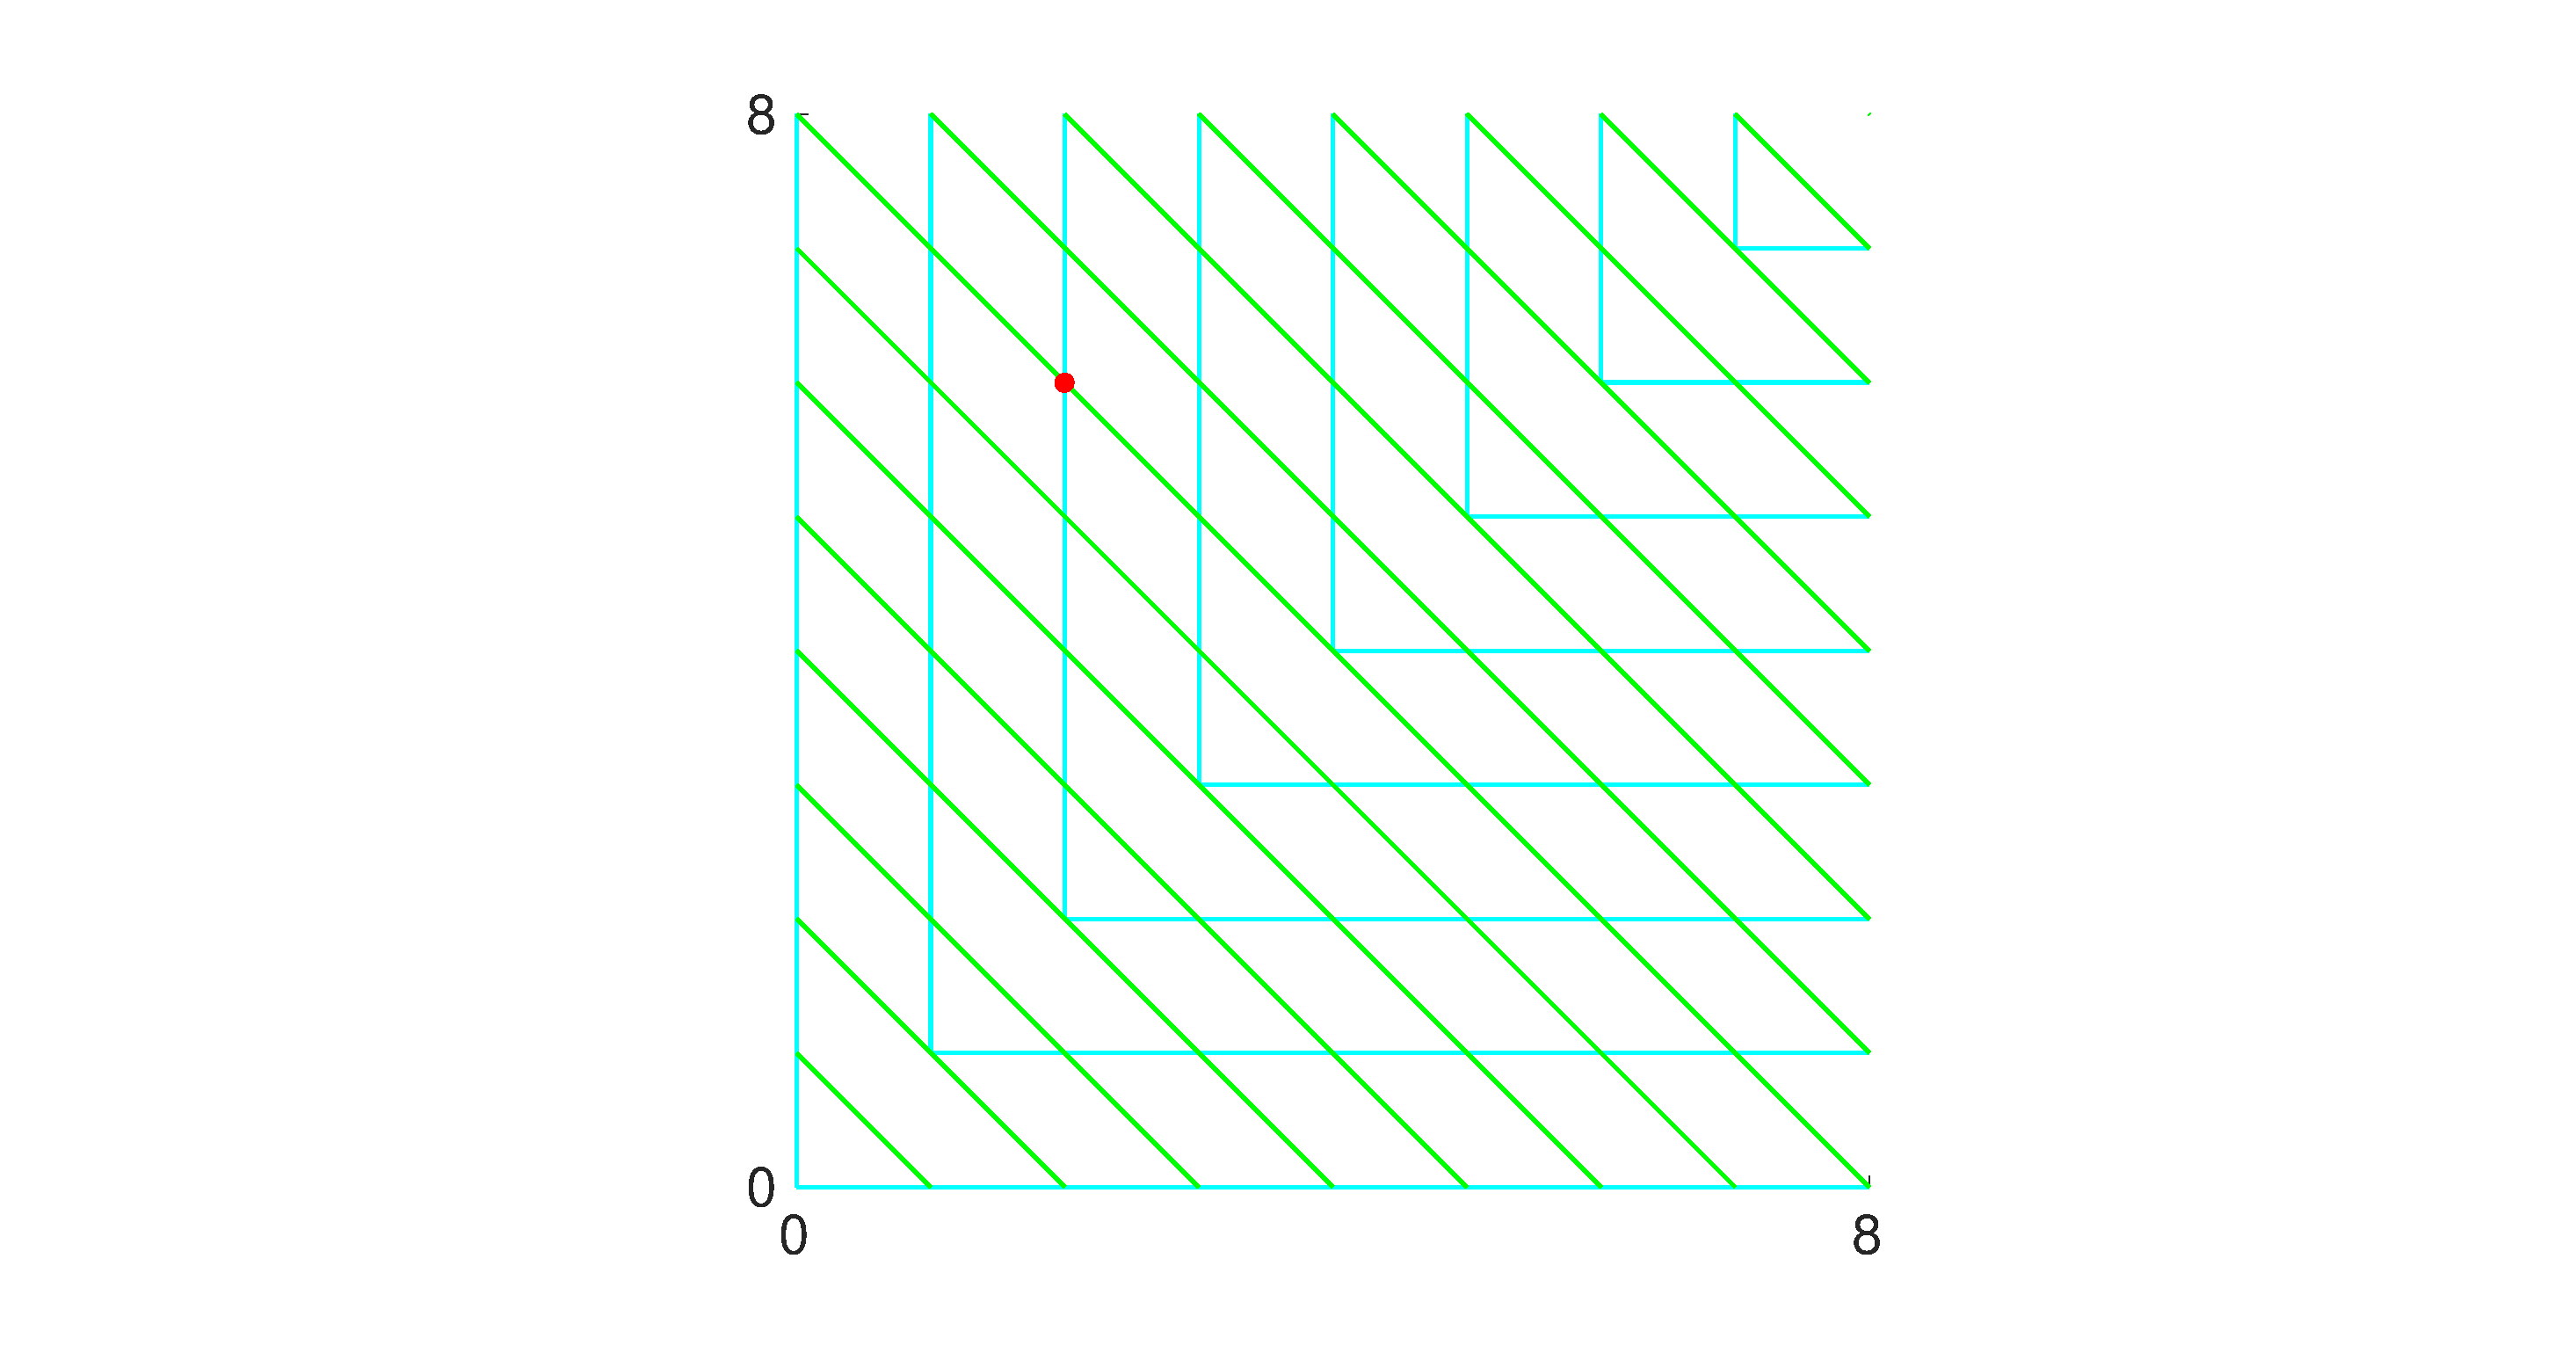
\includegraphics[width=12cm]{figure3.eps}\\
	\caption{Edgeworth box of Ann and Bob}
	\label{Edgeworth}
\end{figure}


\subsection{Part 2}
The Perato optimal allocations happen when Ann's and Bob's indifference curves become tangent. Here since Ann's indifference curve has a kink, being tangent means that Bob's indifferenc curve passes the corner of Ann's curve. Therefore, the contract curve contains all the points having $x=y$. At these points, it is impossible to make both Ann and Bob better off by exchanging goods. The contrast curve is drawn in Fig.\ref{Edgeworth}.

\subsection{Part 3}
For Ann, we need to maximize $U_A=\min(x_A,y_A)$ subject to the constraint that $x_AP_x+y_AP_y=I_A$. Due to the perfect complement property of $x_A$ and $y_A$, utility maximization happens when $x_A=y_A$. Therefore, we have $x_A=y_A=I_A/(P_x+P_y)$.

For Bob, we need to maximize $U_B=x_B+y_B$ subject to the constraint that $x_BP_x+y_BP_y=I_B$. Since $\frac{\partial U_B/\partial x_B}{\partial U_B/\partial y_B}=-1$ is fixed, only when $P_x/P_y=1$ do we have an interior solution. Otherwise, we have corner solutions.

When $P_x=P_y=P$, the budget constraint becomes $x_B+y_B=I_B/p$. In this case, no matter what values $x_B$ and $y_B$ take (as long as both are non-negative), the utility is fixed at $U_B=I_B/P$. When $P_x<P_y$, Bob will only consume $x$. So $x_B=I_B/p_x$ and $y_B=0$. When $p_x>p_y$, Bob will only consume $y$. So $x_B=0$ and $y_B=I_B/p_y$.

In conclusion, Ann's uncompensated demand is $d_{x_A}(P_x,P_y,I_A)=d_{y_A}(P_x,P_y,I_A)=I_A/(P_x+P_y)$. Bob's uncompensated demand is $d_{x_B}(P_x,P_y,I_B)=\displaystyle\left\{\begin{array}{ll}I_B/P_x&(P_x<P_y)\\C&(P_x=P_y)\\0&(P_x>P_y)\end{array}\right.$ and $d_{y_B}(P_x,P_y,I_B)=\displaystyle\left\{\begin{array}{ll}0&(P_x<P_y)\\I_B/p-C&(P_x=P_y)\\I_B/P_y&(P_x>P_y)\end{array}\right.$, where $C$ is an arbitrary value in $[0,I_B/P]$ when $P_x=P_y=P$.

\subsection{Part 4}
The equilibrium point must be on the contract curve, i.e., the diagonal of the Edgeworth box. Moreover, it is on the budget constaint curve that passes through the initial endowment. This curve should be tangent to both Ann's and Bob's indifference curve at the same tangent point. This tangent point is exactly the equilibrium point.

Since Bob's indifference curve is constant sloped, the budget constraint curve tangent to it must overlap with it. Thus this curve has a slope of $-1$. Since it passes through $(x_B,y_B)=(6,2)$, its formula is $x_B+y_B=8$. Expressed in terms of $x_A$ and $y_A$, its formula is $x_A+y_A=8$. The price ratio is $P_x/P_y=-dy/dx=1$.

The equilibrium consumption of Ann is obtained by setting $x_A=y_A$, which gives $(x_A,y_A)=(4,4)$. Since the market is cleared, the equilibrium consumption of Bob is $(x_B,y_B)=(4,4)$.

\subsection{Part 5}
I re-draw the Edgeworth box below, indicating the competitive equilibrium prices, and indifference curves through the initial endowments and through the equilibrium consumption bundles. See Fig.\ref{EdgeworthNew}
\begin{figure}[!htbp]
	\centering
	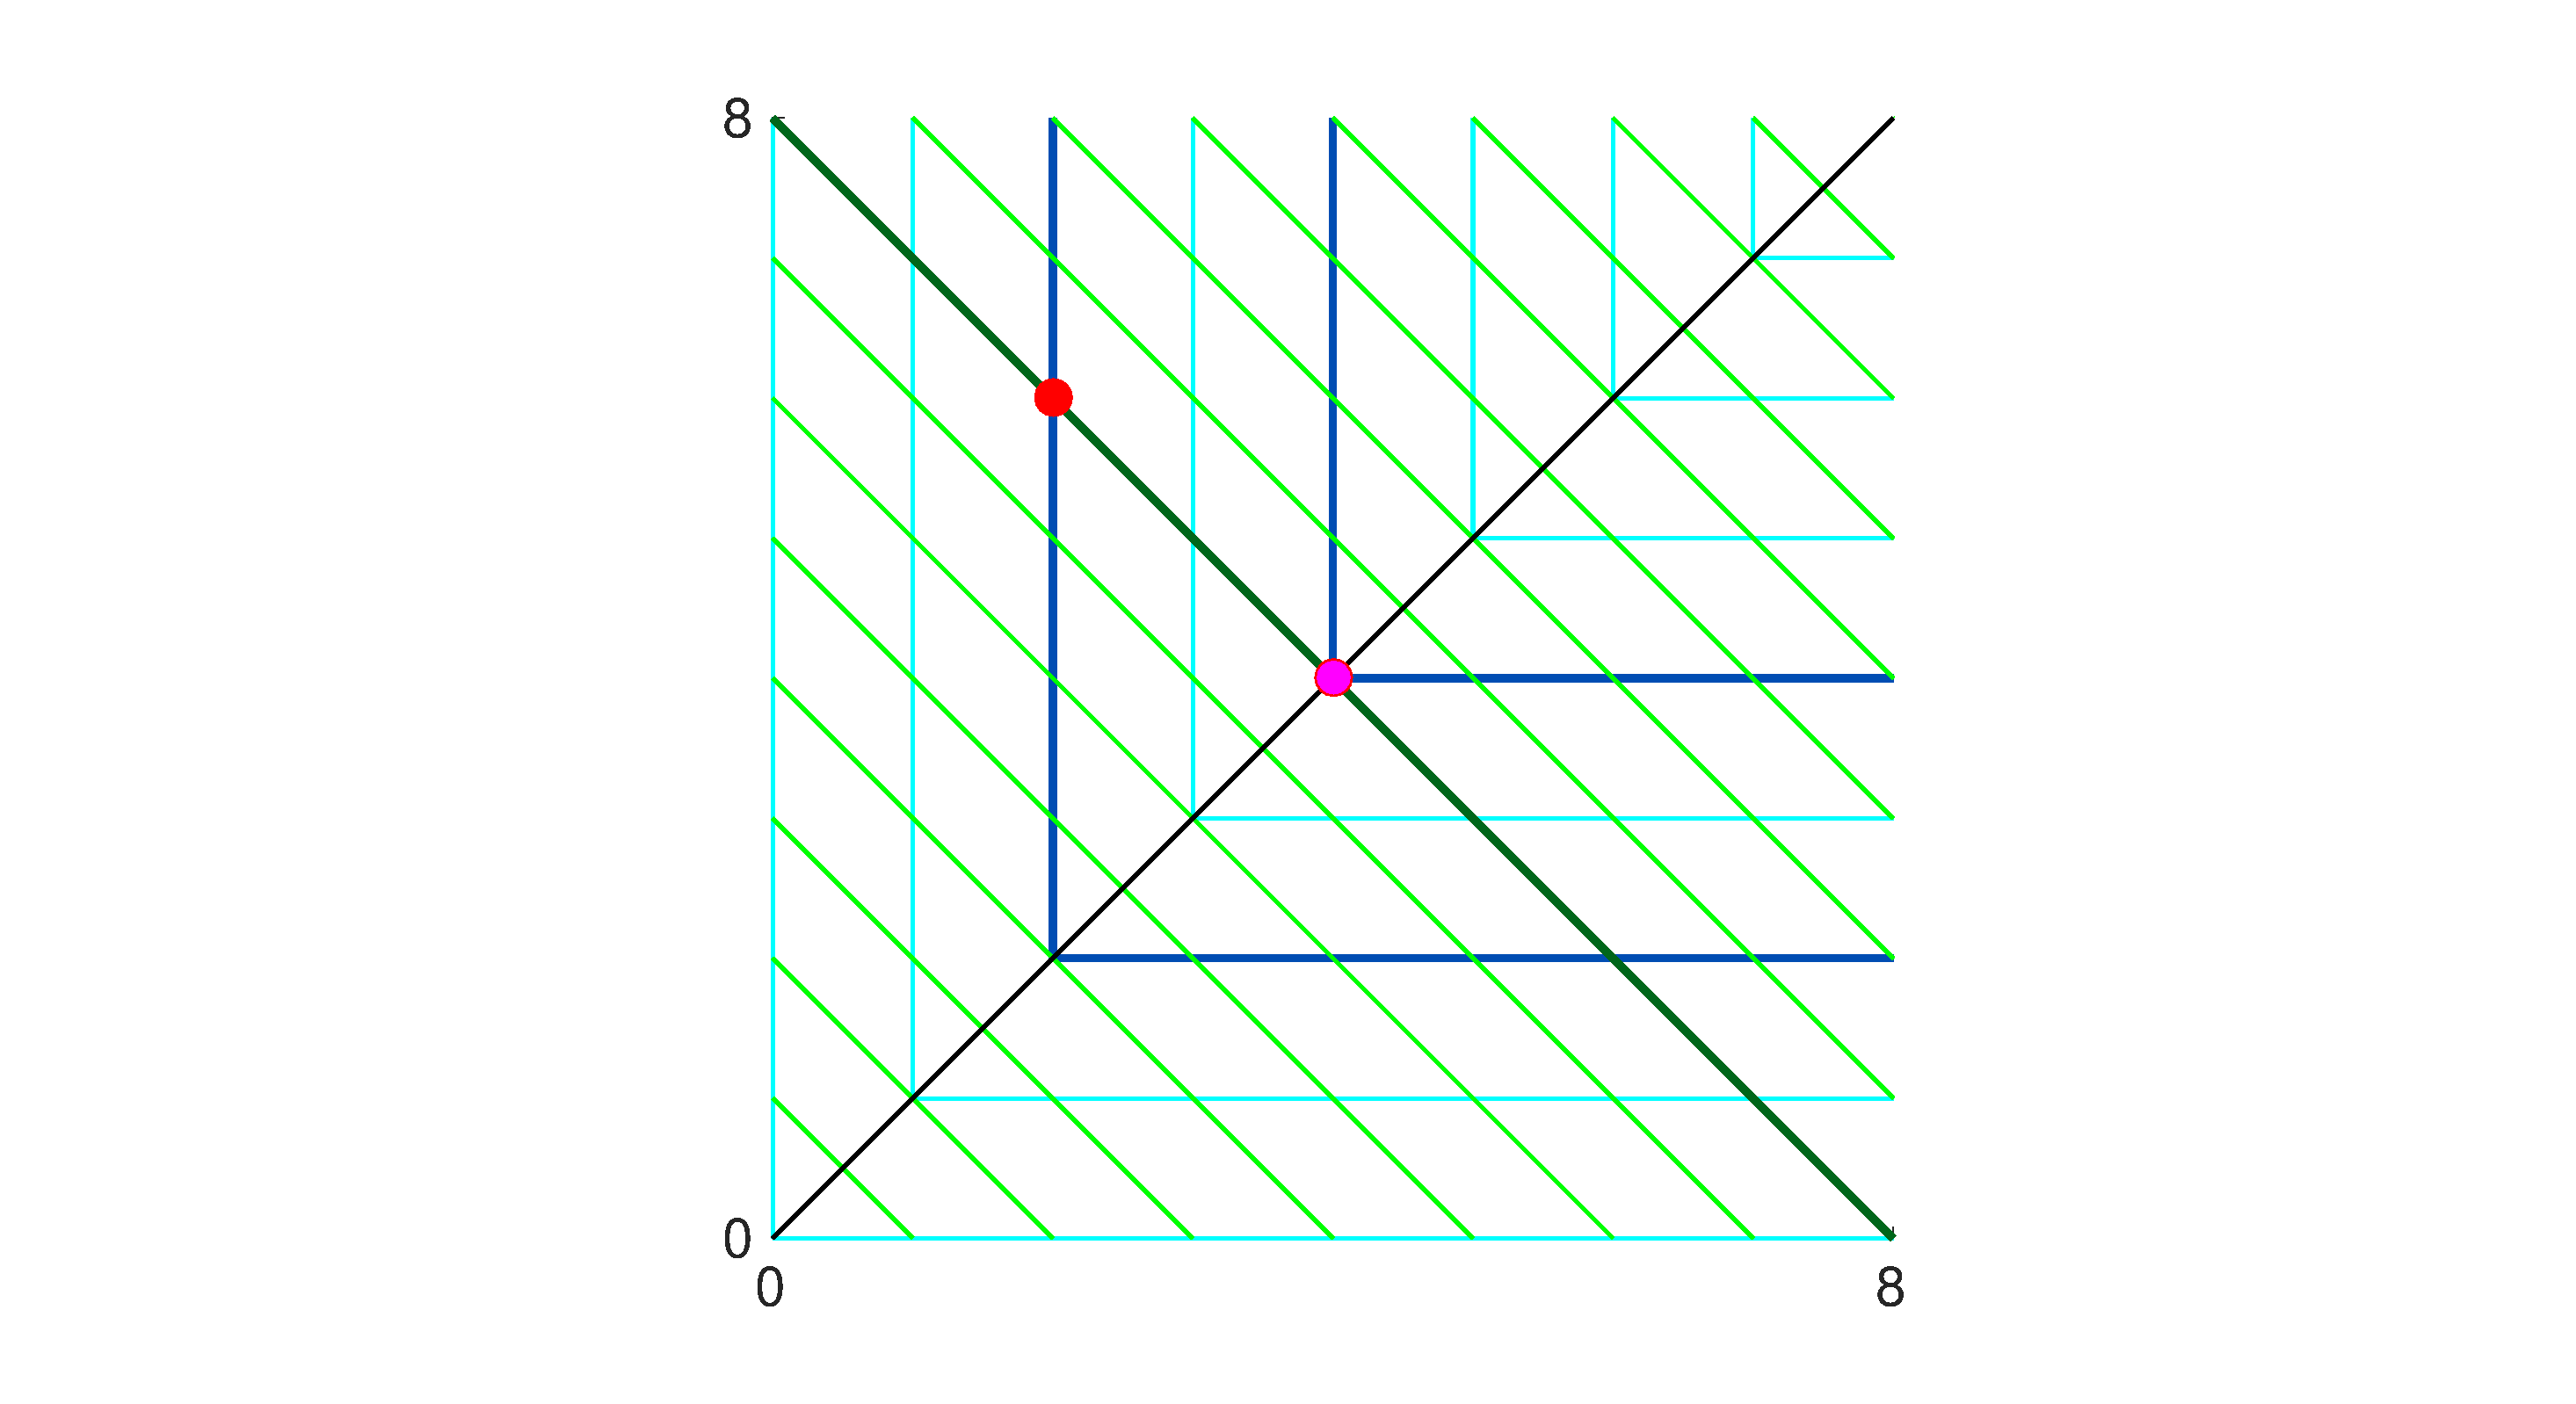
\includegraphics[width=12cm]{figure4.eps}\\
	\caption{Edgeworth box of Ann and Bob}
	\label{EdgeworthNew}
\end{figure}

\subsection{Part 6}
Since both Ann's and Bob's indifference curves are tangent with the budget constraint curve at the equilibrium point, there is no ``lens" enclosed. Thus, there cannot be further changes in allocation that make both of them (weakly) better off. As a result, the equilibrium allocation is Pareto efficient.

\section{Price Distortion and Welfare}
\subsection{Part 1}
For simplicity, let $C=commision$. Let the superscript $i$ denote the city: either $NY$ or $B$.
\begin{align*}
	E[C^i]&=\frac{N^i}{L^S(E[C^i])}cp^i\\
	&=\frac{10\%N^ip^i}{1000E[C^i])}\\
	E[C^i]&=0.01\sqrt{N^ip^i}
\end{align*}

Therefore, the equilibrium wage for each market is
\begin{align*}
	&E[C^{NY}]=0.01\sqrt{N^{NY}p^{NY}}=2\sqrt{10}\approx6.32\\
	&E[C^B]=0.01\sqrt{N^Bp^B}=1
\end{align*}

The number of brokers in each market state is
\begin{align*}
	&L^{S,NY}=1000E[C^{NY}]=2000\sqrt{10}\approx6325\\
	&L^{S,B}=1000E[C^B]=1000
\end{align*}

The surplus of sellers
\begin{align*}
	&S^{S,NY}=(1-c)N^{NY}p^{NY}=3.6\times 10^5\\
	&S^{S,B}=(1-c)N^Bp^B=9\times 10^3
\end{align*}

The surplus of brokers
\begin{align*}
	&S^{B,NY}=cN^{NY}p^{NY}=4\times 10^4\\
	&S^{B,B}=cN^Bp^B=1\times 10^3
\end{align*}

\subsection{Part 2}
In the competitive market, $L^{S,NY}=N^{NY}=4000$ and $L^{S,B}=N^B=1000$. Therefore, the commission in each market is
\begin{align*}
	&C^{NY}=L^{S,NY}/1000=4\\
	&C^B=L^{S,B}/1000=1
\end{align*}

The surplus of sellers
\begin{align*}
	&S^{S,NY}=N^{NY}(p^{NY}-C^{NY})=3.84\times 10^5\\
	&S^{S,B}=N^B(p^B-C^B)=9\times 10^3
\end{align*}

The surplus of brokers
\begin{align*}
	&S^{B,NY}=N^{NY}C^{NY}=1.6\times 10^4\\
	&S^{B,B}=N^BC^B=1\times 10^3
\end{align*}

The deadweight loss of a fixed commission market comes from the fact that, more brokers enter the market compared with the competitive market, but they do the same amount of work in total, in other words, they sell the same number of houses. The deadweight loss equals the opportunity cost of these extra brokers. In the competitive market, they quit the real estate market and turn to other things that can create value to the society.

For the New York market, the deadweight loss is the area of the shaded region in Fig.\ref{DWL}.
\begin{figure}[!htbp]
	\centering
	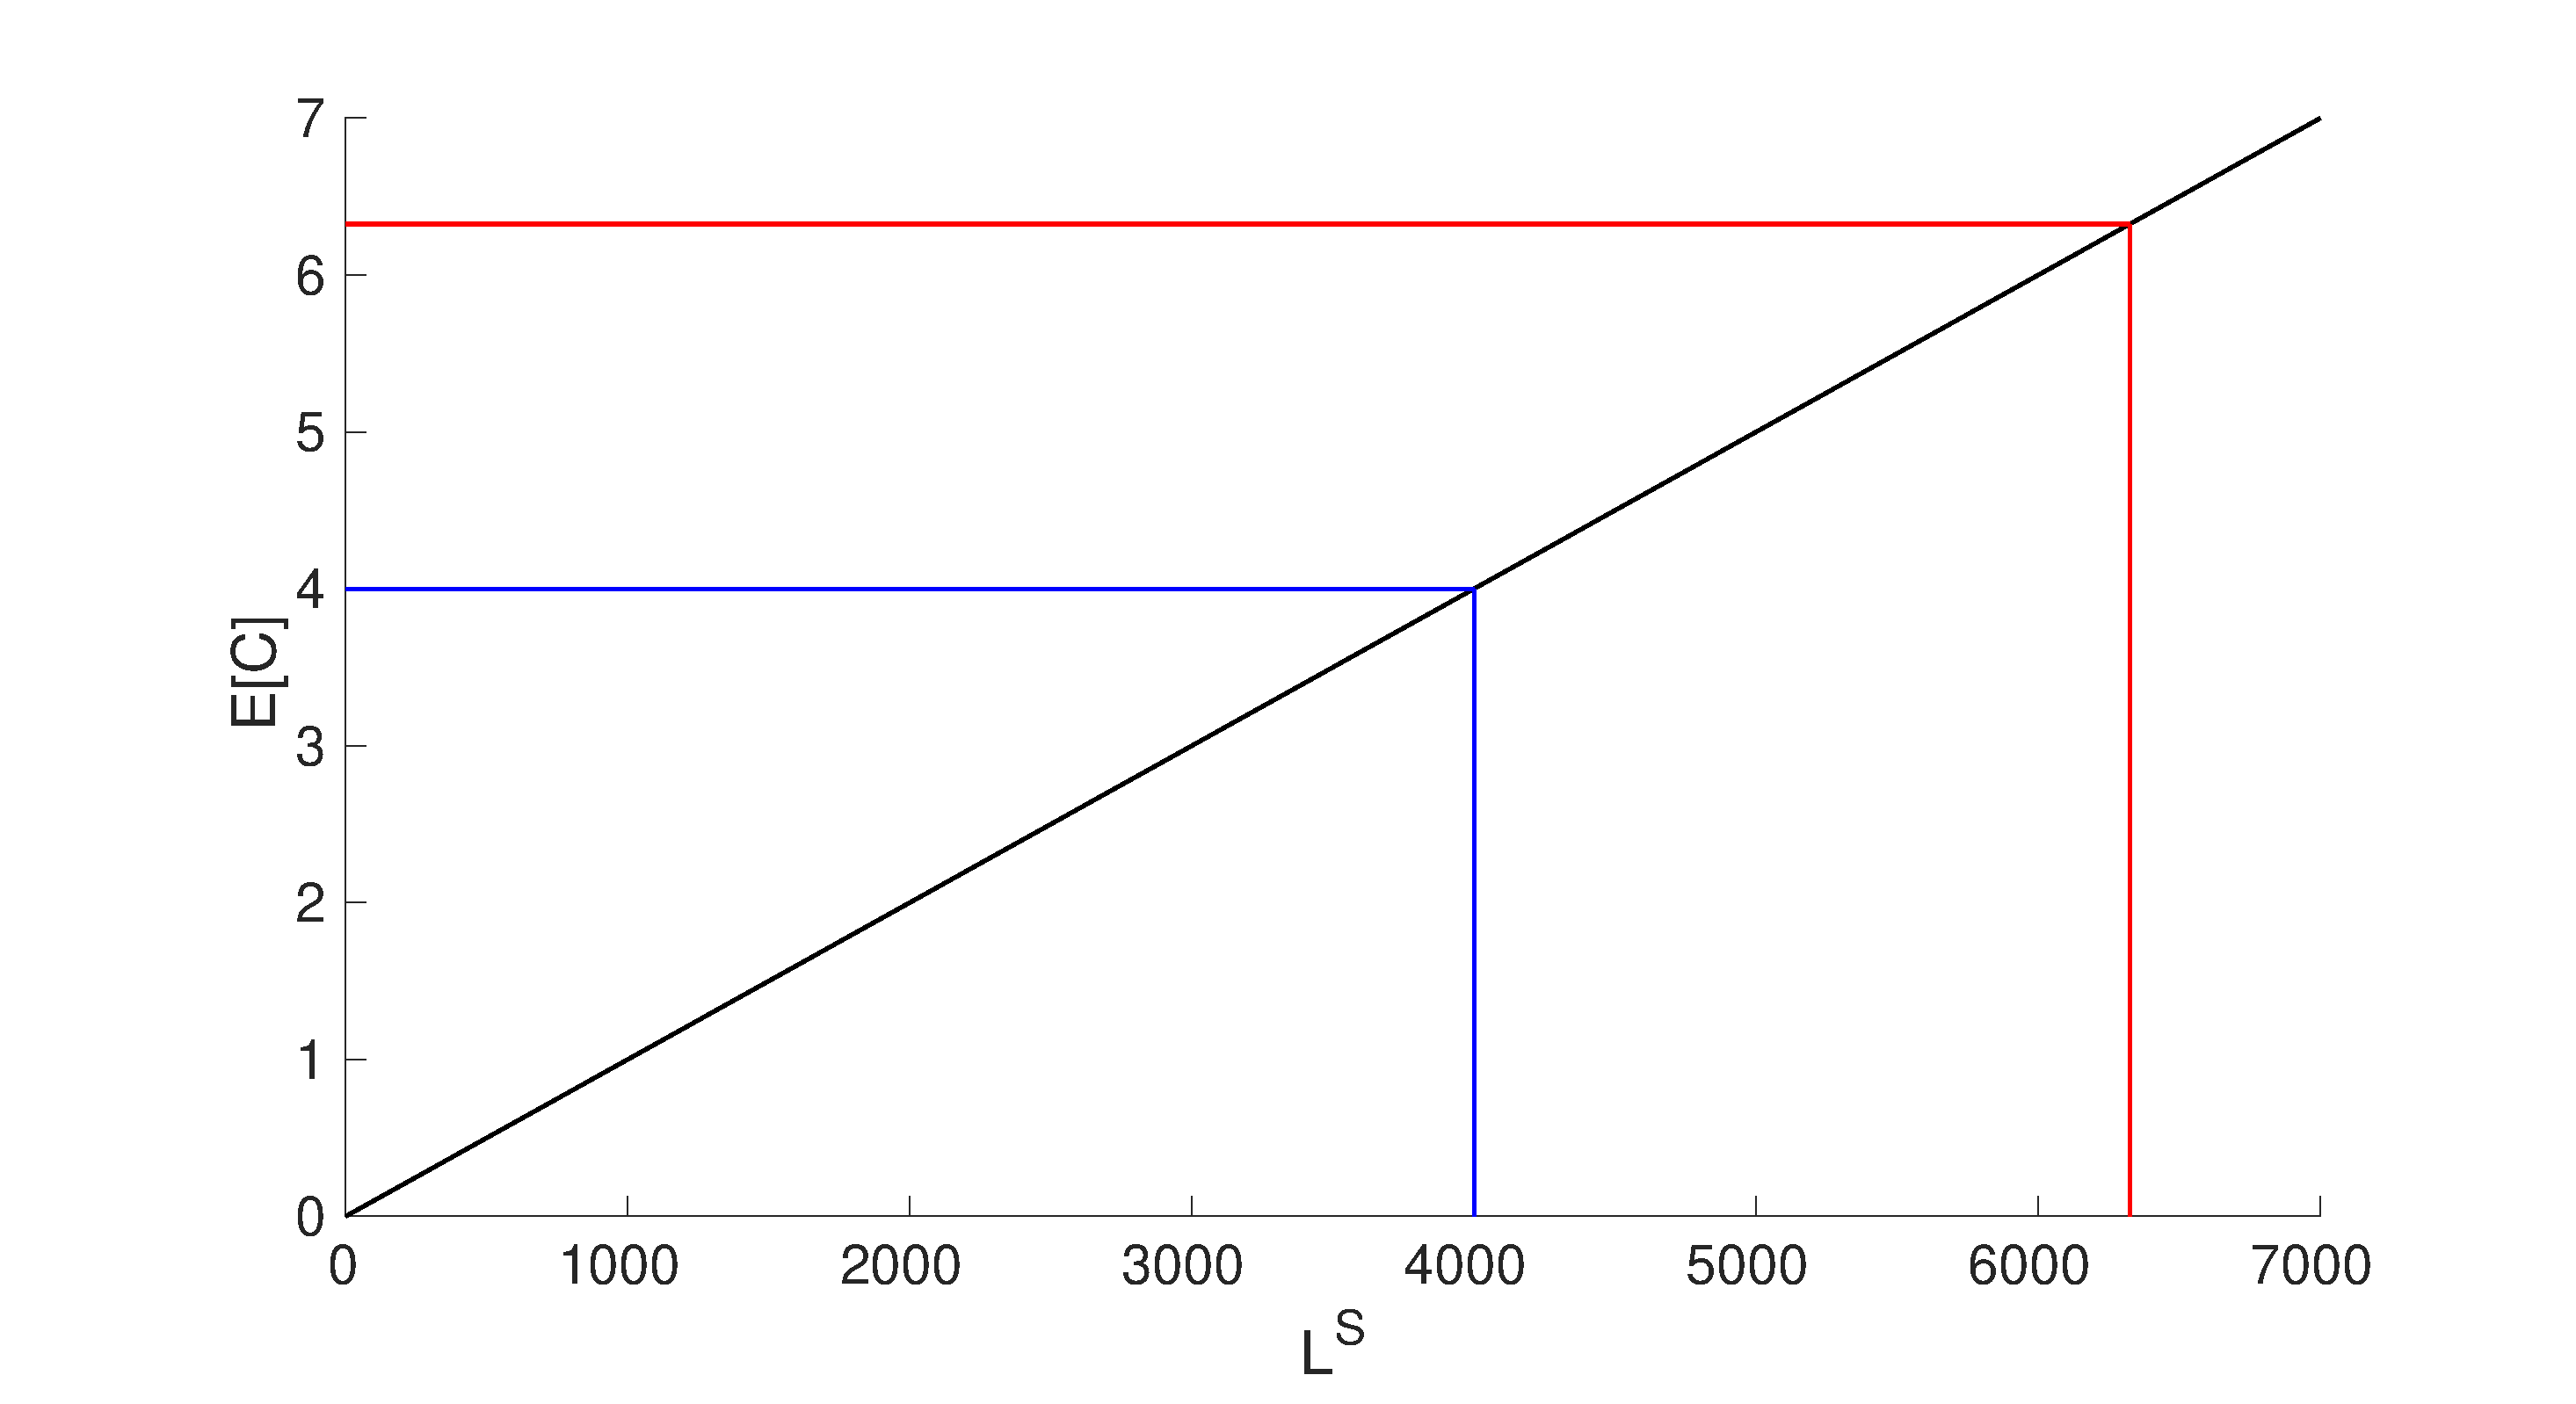
\includegraphics[width=12cm]{figure5.eps}\\
	\caption{Deadweight loss in New York real estate market}
	\label{DWL}
\end{figure}

Therefore,
\begin{equation*}
	DWL^{NY}=(2\sqrt{10}+4)(2000\sqrt{10}-4000)/2=1.2\times 10^4
\end{equation*}

For Boston, however, since there are no excess brokers in the fixed commission market, deadweight loss vanishes. $DWL^B=0$.

\subsection{Part 3}
Lower skilled brokers does less work but shares the commission with others. If they are not in the market, they can probably create more values in other fields that they are better at. Therefore, I believe more social resource is wasted if there are skill differences across brokers. This is an upward bias.

\subsection{Part 4}
Let the treatment be implementation of a fixed commission ($X=1$ for fixed commission and $X=0$ for competitive market). Let the observable $Y$ be the average time houses spend on the market. First consider the city of New York, which represents the boom times. Leave the real estate market in its fixed commission mode and measure $E[Y_{1,NY}|X_{NY}=1]$. Then introduce a policy that forbids fixed commission and measure $E[Y_{0,NY}|X_{NY}=0]$. Calculate $\Delta Y_{NY}=E[Y_{1,NY}|X_{NY}=1]-E[Y_{0,NY}|X_{NY}=0]$. This is the causal effect of a fixed commission on quality dimension during boom times.

In order to make a DID measurement, we do the same thing to the Boston real estate market, parallel to that in New York. We measure $E[Y_{1,B}|X_B=1]$ before the policy and $E[Y_{0,B}|X_B=0]$ after the policy. The difference $\Delta Y_B=E[Y_{1,B}|X_B=1]-E[Y_{0,B}|X_B=0]$ is the causal effect of a fixed commission on quality dimension during non-boom times.

The measurements before and after the policy may involve some time effects since they do not happen in the same background environment. By doing a DID we can reduce this time effect. So we calculate $DID=\Delta Y_{NY}-\Delta Y_B=(E[Y_{1,NY}|X_{NY}=1]-E[Y_{0,NY}|X_{NY}=0])-(E[Y_{1,B}|X_B=1]-E[Y_{0,B}|X_B=0])$. The magnitude of the result shows the importance of quality dimension. In other words, a bigger DID means more low skilled brokers entering the market, and thus a bigger deadweight loss, in the boom times.

\end{document}
